\documentclass[11pt]{article}
\renewcommand{\baselinestretch}{1.05}
\usepackage{amsmath,amsthm,verbatim,amssymb,amsfonts,amscd, graphicx}
\usepackage{graphics}
\usepackage{epstopdf}
\usepackage{float}
\usepackage{geometry}
\geometry{legalpaper, margin=.25in}
%\usepackage{tikz}
%\usepackage{tikz-3dplot}
%\usepackage{pgfplots}
%\pgfplotsset{width=9 cm,compat=1.9}
%\usepgfplotslibrary{external}
%\tikzexternalize
\newcommand\Z{{\mathbb Z}}
\newcommand\F{{\mathbb F}}
\newcommand\N{{\mathbb N}}
\newcommand\R{{\mathbb R}}
\newcommand\Q{{\mathbb Q}}
\newcommand\C{{\mathbb C}}
\topmargin0.0cm
\headheight0.0cm
\headsep0.0cm
\oddsidemargin0.0cm
\textheight23.0cm
\textwidth16.5cm
\footskip1.0cm
\theoremstyle{plain}
\newtheorem{theorem}{Theorem}
\newtheorem{corollary}{Corollary}
\newtheorem{lemma}{Lemma}
\newtheorem{proposition}{Proposition}
%\newtheorem*{surfacecor}{Corollary 1}
\newtheorem{conjecture}{Conjecture} 
\newtheorem{question}{Question} 
\theoremstyle{definition}
\newtheorem{definition}{Definition}

 \begin{document}
 

\pagenumbering{gobble}
\title{How Firms Hire Workers: Graph Matching and the Labor Market}
\author{Elizabeth Maloney}
%\maketitle
\begin{figure}[H]
\begin{center}
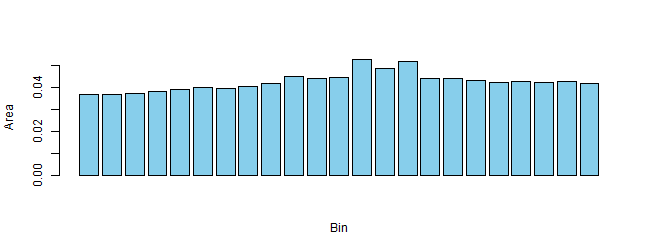
\includegraphics[trim ={3.5cm 2.7cm 2cm 2cm},scale=.6, clip=true]{Binned_Areas13.png}
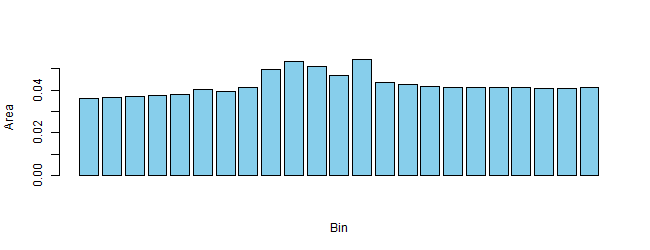
\includegraphics[trim ={3.5cm 2.7cm 2cm 2cm},scale=.6, clip=true]{Binned_Areas14.png}
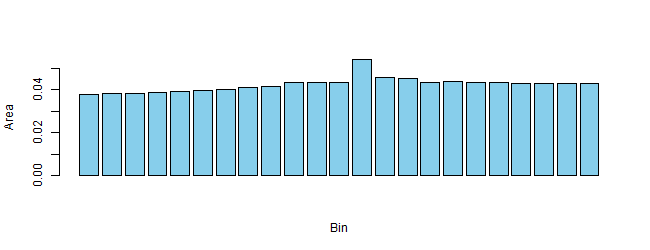
\includegraphics[trim ={3.5cm 2.7cm 2cm 2cm},scale=.6, clip=true]{Binned_Areas15.png}
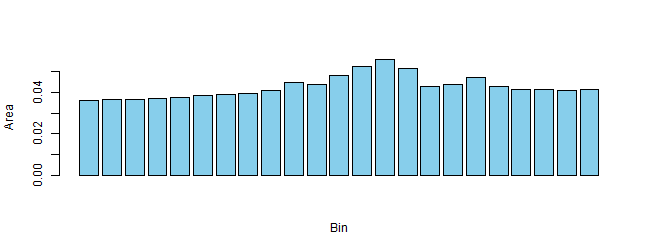
\includegraphics[trim ={3.5cm 2.7cm 2cm 2cm},scale=.6, clip=true]{Binned_Areas16.png}
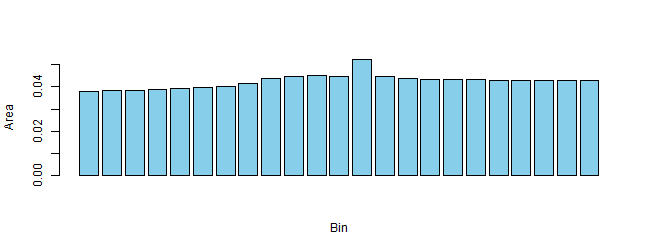
\includegraphics[trim ={3.5cm 2.7cm 2cm 2cm},scale=.6, clip=true]{Binned_Areas17.png}
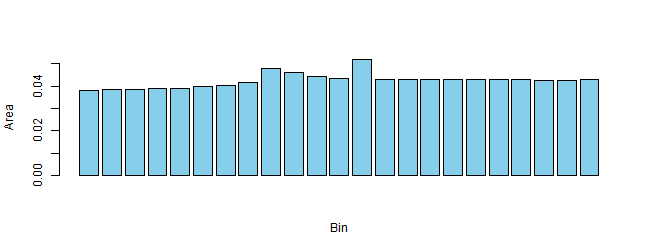
\includegraphics[trim ={3.5cm 2.7cm 2cm 2cm},scale=.6, clip=true]{Binned_Areas18.png}
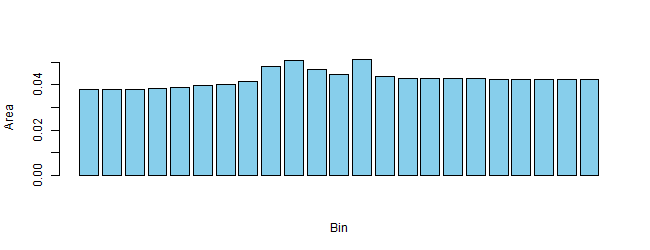
\includegraphics[trim ={3.5cm 2.7cm 2cm 2cm},scale=.6, clip=true]{Binned_Areas19.png}
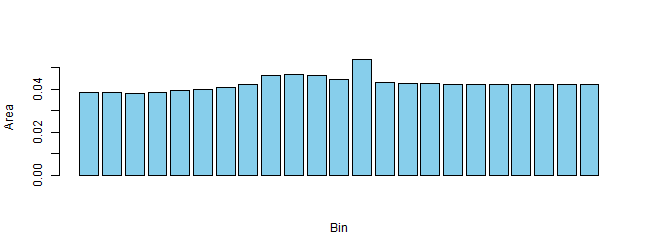
\includegraphics[trim ={3.5cm 2.7cm 2cm 2cm},scale=.6, clip=true]{Binned_Areas20.png}
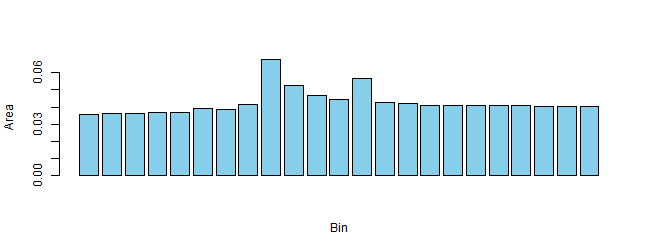
\includegraphics[trim ={3.5cm 2.7cm 2cm 2cm},scale=.6, clip=true]{Binned_Areas21.png}
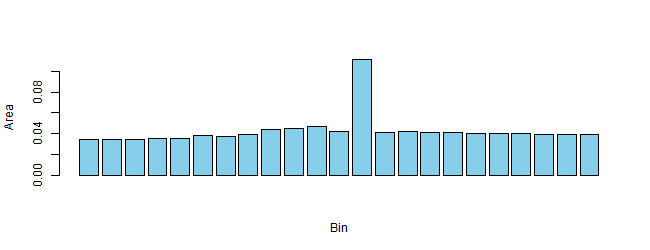
\includegraphics[trim ={3.5cm 2.7cm 2cm 2cm},scale=.6, clip=true]{Binned_Areas22.png}
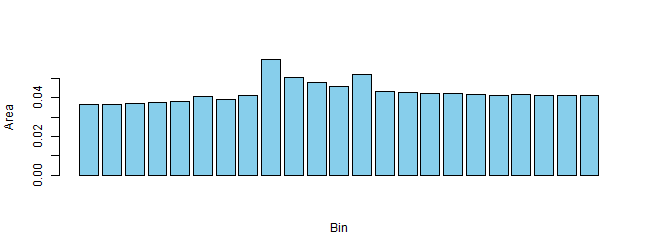
\includegraphics[trim ={3.5cm 2.7cm 2cm 2cm},scale=.6, clip=true]{Binned_Areas23.png}
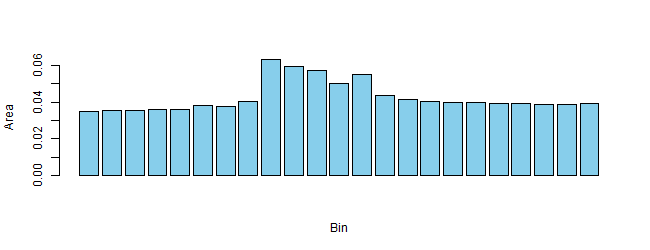
\includegraphics[trim ={3.5cm 2.7cm 2cm 2cm},scale=.6, clip=true]{Binned_Areas24.png}
\end{center}
\end{figure}
\end{document}




\end{document}